\subsection{Calculation of water height}
First, the function computes the water height present at the top of the surface unit. This value is composed with rainfall height $P$ (in $m$) and runoff output discharge $Q_{SU}(t-1)$ (in $m\up3/s$) from potential upper connected SUs calculated at the previous simulation time step.

\begin{equation}
\label{HeightSU}
H = P + \sum_{SU_{up}} \left( \frac{Q_{SU}(t-1) \times \Delta t}{A_{SU}} \right)
\end{equation}


where $H$ is the water height present at the surface of the SU ($m$), $\Delta t$ is the simulation time step ($s$), and $A_{SU}$ is the area of the unit on which the calculation is done ($m\up2$).


\subsection{Calculation of infiltrability}
The ``\englishname'' \cite{MorelS1978} is a modification of Green and Ampt's \cite{Green1911} equation. The main assumption is the rectangular form of the wetting front trough the soil, as schematized hereafter. Then, the model was adapted to the MHYDAS structure by Moussa and al. \cite{Moussa2002}.\\

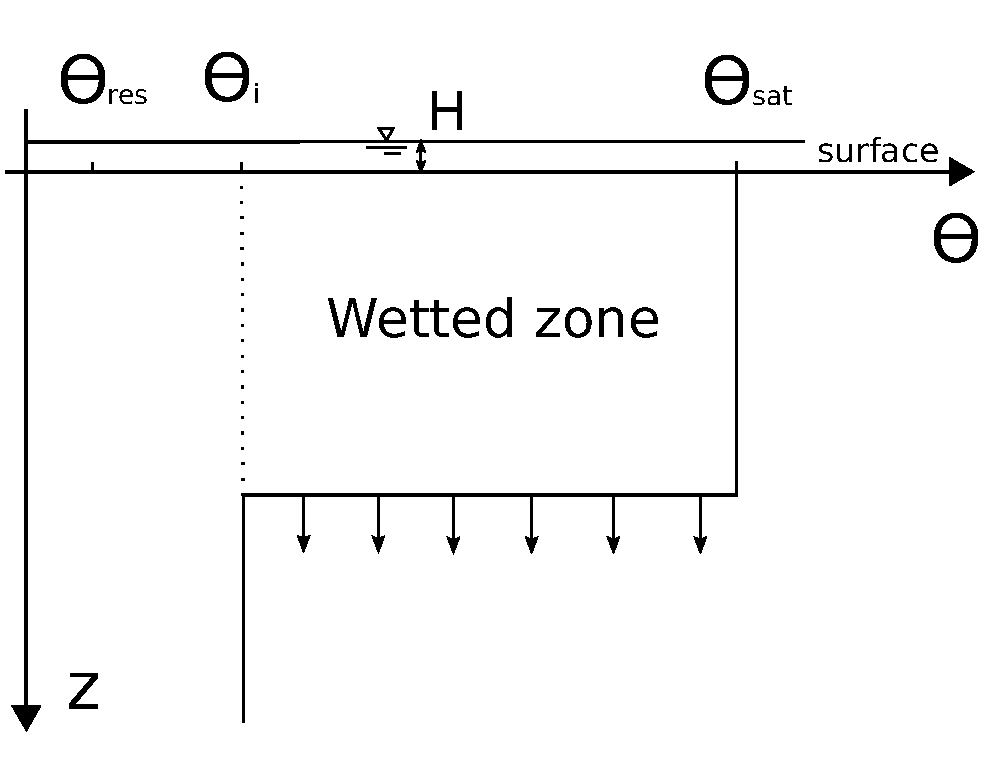
\includegraphics[width=8cm]{doc/common/Green_Ampt_humidity.pdf}

Runoff cannot occur as long as the soil surface retention potential is not reached. Therefore, at every time step, the model needs to determine whether the ponding time ($t_p$) has been reached. For $t < t_p$ all the rain is infiltrated and for $t > t_p$ the cumulative infiltration $F(t)$ is calculated from the equation \ref{MSeytoux}. This behaviour could be represented with the infiltratbility $f(t)$ ($m/s$) which dicrease in time from $t_p$. Then, the value of $f(t)$ tends towards the saturated hydraulic conductivity $K_{sat}$.\\

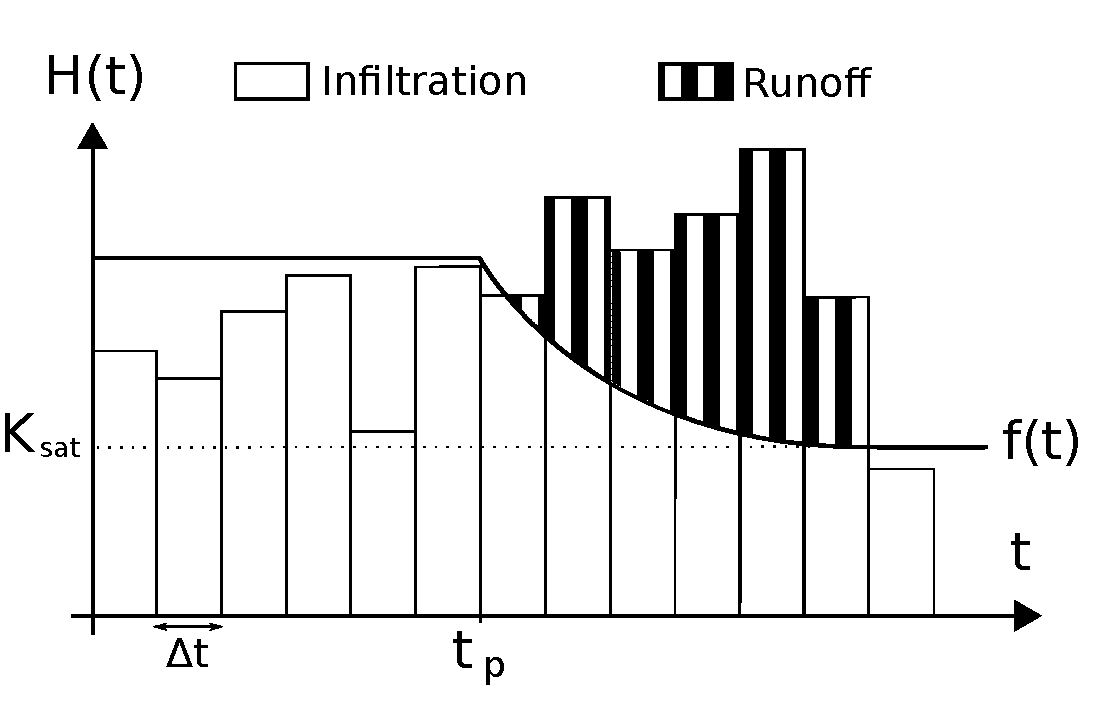
\includegraphics[width=8cm]{doc/common/Separation_infiltration_ruissellement_MSeytoux.pdf}
\begin{equation}
\label{MSeytoux}
\begin{array}{l}
F(t) - F_p - \left(S_f + F_p \times \left(1 - \frac{1}{\beta_{MS}} \right) \right) \times ln \left(\frac{S_f + F(t)}{S_f+F_p} \right)\\
\\
 = \frac{K_s \times (t - t_p)}{\beta_{MS}}
\end{array}
\end{equation}


where $F_p$ is the cumulative infiltration when ponding occurs ($m$), $\beta_{MS}$ is the viscous correction parameter ($-$) ranged between 1 and 1,7 and usually taken equal to 1,3 \cite{MorelS1984}, $K_s$ is the saturated hydraulic conductivity ($m/s$). $K_s$ is a distributed parameter on surface units but it can be time variable as a function of soil practice and rainfall.\\

The parameter $S_f$ is a factor composed of storage and suction ($m$). This factor is calculated with the equation \ref{Sf_equation} which is an approximation of the ``suction head / water content'' relation curve $\phi(\theta)$, hereafter.\\

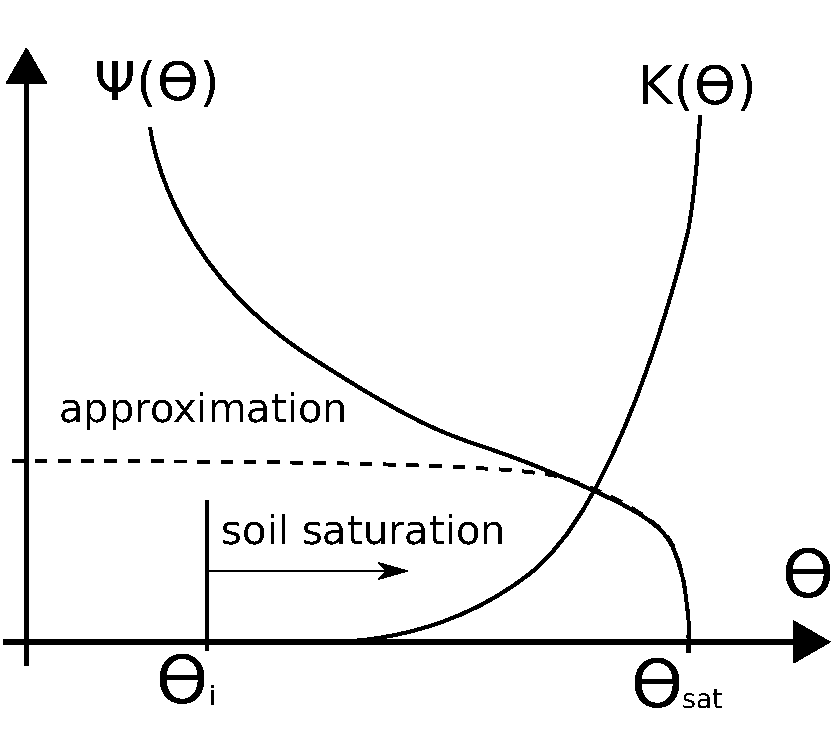
\includegraphics[width=8cm]{doc/common/Sf_approximation.pdf}
\begin{equation}
\label{Sf_equation}
S_f=(\theta_s-\theta_i)\times H_c \times \left(1-\frac{1}{3}\times \left( \frac{\theta_i-\theta_r}{\theta_s-\theta_r} \right) ^6 \right)
\end{equation}


where $Hc$ is the capillary height ($m$), $\theta_s$  is the volumetric soil water content at saturation ($m\up3/m\up3$), $\theta_r$ is the volumetric residual soil water content ($m\up3 /m\up3$) and $\theta_i$ is the initial water content in the top surface layer ($m\up3 /m\up3$). This calculation is done once at the beginning of the simulation.\\

To determine the cumulative infiltration $F(t)$ at every time step, the function realizes iterations to satisfy the equation \ref{MSeytoux}. The parameter $ResStep$ ($m$) characterises the accuracy of calculated cumulative infiltration value. The smaller this parameter is, the more accurate the value $F$ is. However, simulation duration is higher because of the greater number of iteration steps.


\subsection{Calculation of infiltration and runoff}
Then, produced variables are calculated as following :\\

\hspace{-0.53cm} if $t \le t_p$ : \ \ \ \begin{equation}
\left\{ \begin{array}{l}
   I = H\\
   R = 0
  \end{array}
\right.
\end{equation}\\
\vspace{-0.5mm}
if $t > t_p$ : \ \ \ \begin{equation}
\left\{ \begin{array}{l}
   I = F(t) - F(t-1)\\
   R = H - \left(F(t) - F(t-1) \right)
  \end{array}
\right.
\end{equation}

where $I$ is the infiltrated water height ($m$), $R$ is the runoff water height on SU ($m$), $F$ is the cumulative infiltration ($m$) at time $t$, and $H$ is the water height at the top of the surface unit ($m$) calculated in equation \ref{HeightSU}.\\

We could note that once $t_p$ is reached, the soil cannot be ``unsaturated''. Therefore, the ``\englishname'' should be only used at the scale of a rain event.\\

Some examples of use are available in the paper of Morel-Seytoux \cite{MorelS1984}, Chahinian \cite{Chahinian2004b} and in thesis of Chahinian \cite{Chahinian2004} and Ghesquière \cite{Ghesquiere2008}.
